\documentclass{acm_proc_article-sp}

\begin{document}

\title{Algorithmic and Economic Aspects of the Internet}
%
% You need the command \numberofauthors to handle the 'placement
% and alignment' of the authors beneath the title.
%
% For aesthetic reasons, we recommend 'three authors at a time'
% i.e. three 'name/affiliation blocks' be placed beneath the title.
%
% NOTE: You are NOT restricted in how many 'rows' of
% "name/affiliations" may appear. We just ask that you restrict
% the number of 'columns' to three.
%
% Because of the available 'opening page real-estate'
% we ask you to refrain from putting more than six authors
% (two rows with three columns) beneath the article title.
% More than six makes the first-page appear very cluttered indeed.
%
% Use the \alignauthor commands to handle the names
% and affiliations for an 'aesthetic maximum' of six authors.
% Add names, affiliations, addresses for
% the seventh etc. author(s) as the argument for the
% \additionalauthors command.
% These 'additional authors' will be output/set for you
% without further effort on your part as the last section in
% the body of your article BEFORE References or any Appendices.

\numberofauthors{2} %  in this sample file, there are a *total*
% of EIGHT authors. SIX appear on the 'first-page' (for formatting
% reasons) and the remaining two appear in the \additionalauthors section.
%
\author{
% You can go ahead and credit any number of authors here,
% e.g. one 'row of three' or two rows (consisting of one row of three
% and a second row of one, two or three).
%
% The command \alignauthor (no curly braces needed) should
% precede each author name, affiliation/snail-mail address and
% e-mail address. Additionally, tag each line of
% affiliation/address with \affaddr, and tag the
% e-mail address with \email.
%
% 1st. author
\alignauthor
Sam Phippen\titlenote{sp9857}\\
       \email{samphippen@googlemail.com}
% 2nd. author
\alignauthor
Luke Murray\titlenote{lm9131}
       \email{lm9131@bris.ac.uk}
}
% There's nothing stopping you putting the seventh, eighth, etc.
% author on the opening page (as the 'third row') but we ask,
% for aesthetic reasons that you place these 'additional authors'
% in the \additional authors block, viz.
% Just remember to make sure that the TOTAL number of authors
% is the number that will appear on the first page PLUS the
% number that will appear in the \additionalauthors section.

\maketitle
\begin{abstract}

For the assignment we attempted to implement the Adaptive
Aggressive\cite{Vytellingum:AA} trading agent strategy. Even with corrections
emailed by D. Cliff we found that our strategy does not trade as efficiently as
is implied in other background research\cite{DC:dominate}. In this paper we've
done a comparative analysis of the existing trading agents provided in BSE,
along with our implementation. We have also performed a post mortem analysis as
to why we believe that our trader is not trading as efficiently as expected.

We had initially set our sights on taking an implementation of AA and trying to
improve upon it, with a view to building something new and potentially more
effective, however, having found ourselves in a position where the agent is
nowhere near as effective as we expected, this was not a good springboard for
extension.

\end{abstract}

\section{Analysis of our agent with existing traders}

\subsection {Many versus many tests} For the analysis we started with a many
versus many test of our implementation versus each of the agents provided with
BSE. In this experiment we used the stepped supply and demand schedule provided
with an early version of the Bristol Stock Exchange, with three distinct time
periods, the first having prices in the range 10-190, the second in the range
200-300 and the third having prices in the same range as the first. In the many
versus many test 20 agents of each type were used (10 sellers and 10 buyers),
and the tests with this supply and demand schedule were repeated a total of 25
times.

The table below shows the number of rounds that our agent lost, the mean
difference in profit between the other agent and ours, and the standard
deviation of the difference in profit also.

\begin{center}
  \begin{tabular}{ l | l | l | l }
        Agent Type & Tests lost & $\Delta$ Profit Mean & $\Delta$ Profit StDev \\\hline
        Giveaway & 24 & 63.84 & 34.16\\
        ZIC & 25 & 75.38 & 36.15\\
        Shaver & 25 & 95.63 & 21.01\\
        Sniper & 25 & 22.67 & 12.78\\
        ZIP & 25 & 97.08 & 41.38\\
  \end{tabular}
\end{center}

In almost all of these cases our agent consistently generated a profit,
however when run against the Shaver agent, an oddity occurred. The agent on
average generated a loss which can be seen on the box plot in figure 1.

\begin{figure}[h!] 
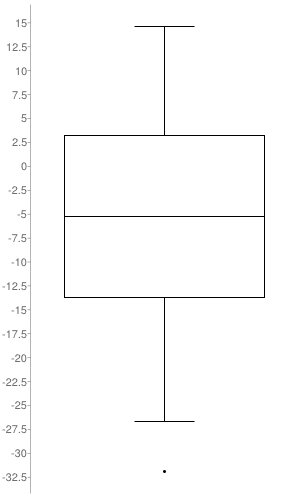
\includegraphics[width=80mm]{box-plot-image.png}

\caption{Box plot of average profits of the 20 AA agents implemented by us in
the many vs many test against shaver agents. Box plot generated from:
http://www.alcula.com/calculators/statistics/box-plot/}
\end{figure}

-- insert explanation about that here.

\subsection{1 v 1 tests}
Given these initially dismal results, we decided that a good place to start a
detailed analysis would be a 1v1 test with the Giveaway trader, which is
clearly the worst of all the traders within the BSE system. 300 1v1 tests were
performed, we used the same schedule as the many versus many test. Results
where both bots made zero profit were eliminated, this brought the number of
tests included for analysis down from 300 to 242. Of these tests 103 were won
by Giveaway and 139 were won by our agent. The distributions of profit for each
agent, as well as the distribution of differences in profit can be seen in the
following histograms.

\begin{figure}[h!] 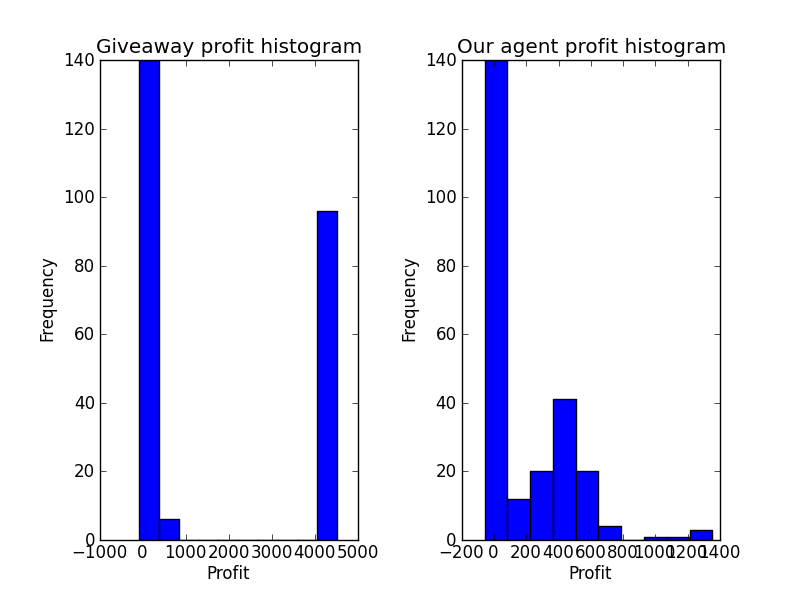
\includegraphics[width=80mm]{giveaway_1_v_1.png}
\caption{Histogram of profit distributions over 300 similar trading runs for
the two bot types used in the 1v1 test. Note axis are different for the two
bots} \end{figure}

\begin{figure}[h!] 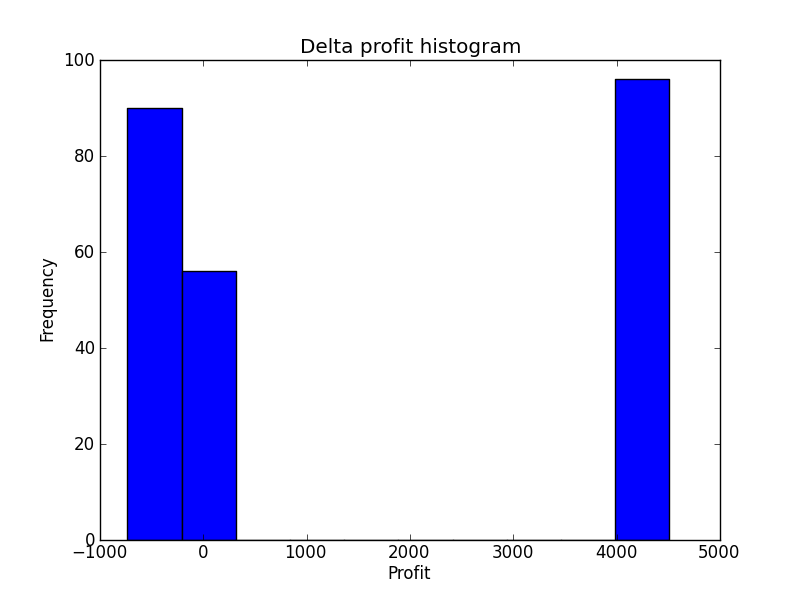
\includegraphics[width=80mm]{giveaway_1_v_1_delta.png}
\caption {Histogram showing the difference between Giveaway and our AA implementation,
positive profit represents cases where Giveaway made more profit than AA}
\end{figure}

\newpage
Upon initially inspecting these graphs we had assumed that our agent should
lose to Giveaway, however we checked the medians of the distributions and noted
that the median profit of the Giveaway agent (1.7) was less than the median
profit (50.0) of our agent. We feel that this difference in profits is the
reason for our agent's overall victory against Giveaway. To determine if the
difference in medians is significant we decided to use the Wilcoxon signed-rank
test\cite{wiki:wilcoxon}. We like this test because:

\begin{enumerate}
\item It makes no assumptions about the underlying
distribution of profit pairs, as we can see from the histogram, these are
nowhere near normally distributed.

\item It handles the fact that the pairs are dependant but the individual runs
are independent.

\item We feel that the assumptions the distribution makes are fulfilled here:
the pairs do come from the same distributions. The pairs have been generated
largely at random by running different tests and collecting results. The data
are obviously ordinal as they are floating amounts of profit.

\end{enumerate}

In order to conduct this test we represented each run as a pair of
$(profit_{giveaway}, profit_{agent})$. The profits in the pair are taken from
the average profit column in the output of running BSE, so in fact the profit
values are divided by two, because their are two of each agent running in the
system. This will not effect the output of the test, as the change in magnitude
is the same for both agents. The test runs over the difference between the
first and second value in the pair. Our null hypothesis $H0$ is that the median
difference of each pair is zero, with our positive hypothesis $H1$ being that
the median difference of each pair is not zero. We performed the test using
scipy's built in Wilcoxon signed-rank test implementation\cite{scipy:wilcoxon}
and the results were extremely conclusive.  With $p=1.2\times10^{-6}$ we reject
$H0$ and conclude that the difference in medians is significant, as such the
profits generated by our agent are significantly better than Giveaway's.

This test was repeated for each of ZIC, Shaver, Sniper and ZIP. In each case
the results were that our bot performed significantly worse than the other agent (p < 0.01
in each case).

\subsection{One in many tests}
We also evaluated the agent initially in a one versus many test against a ZIC
trader which gave better results. Using a similar strategy above we started
with 25 tests to determine winners and average profits, however the results
were not totally conclusive, so we decided to generate some 300 experimental
results in order to attempt to draw conclusions about whether the bot performs
better in one v many tests. The results are shown below, using the same supply
and demand schedule, and two of our agent (1 buyer, 1 seller) and 20 of
the other agent (10 buyers, 10 sellers):

\begin{center}
\begin{tabular}{ l|l|l|l }
Agent Type & Tests lost & $\Delta$ Profit Mean & $\Delta$ Profit StDev \\
\hline
Giveaway & 157 & -2.28 & 86.95\\ 
ZIC & 225 & 52.86 & 83.99\\ 
Shaver & 287 & 76.36 & 46.06\\ 
Sniper & 256 & 19.49 & 16.74\\ 
ZIP & 234 & 64.76 & 89.76
\end{tabular}
\end{center}

We can see here that the agent performs better when trading on it's own than in
a small swarm.

You can use whatever symbols, accented characters, or
non-English characters you need anywhere in your document;
you can find a complete list of what is
available in the \textit{\LaTeX\
User's Guide}\cite{Lamport:LaTeX}.

\subsection{Math Equations}
You may want to display math equations in three distinct styles:
inline, numbered or non-numbered display.  Each of
the three are discussed in the next sections.

\subsubsection{Inline (In-text) Equations}
A formula that appears in the running text is called an
inline or in-text formula.  It is produced by the
\textbf{math} environment, which can be
invoked with the usual \texttt{{\char'134}begin. . .{\char'134}end}
construction or with the short form \texttt{\$. . .\$}. You
can use any of the symbols and structures,
from $\alpha$ to $\omega$, available in
\LaTeX\cite{Lamport:LaTeX}; this section will simply show a
few examples of in-text equations in context. Notice how
this equation: \begin{math}\lim_{n\rightarrow \infty}x=0\end{math},
set here in in-line math style, looks slightly different when
set in display style.  (See next section).

\subsubsection{Display Equations}
A numbered display equation -- one set off by vertical space
from the text and centered horizontally -- is produced
by the \textbf{equation} environment. An unnumbered display
equation is produced by the \textbf{displaymath} environment.

Again, in either environment, you can use any of the symbols
and structures available in \LaTeX; this section will just
give a couple of examples of display equations in context.
First, consider the equation, shown as an inline equation above:
\begin{equation}\lim_{n\rightarrow \infty}x=0\end{equation}
Notice how it is formatted somewhat differently in
the \textbf{displaymath}
environment.  Now, we'll enter an unnumbered equation:
\begin{displaymath}\sum_{i=0}^{\infty} x + 1\end{displaymath}
and follow it with another numbered equation:
\begin{equation}\sum_{i=0}^{\infty}x_i=\int_{0}^{\pi+2} f\end{equation}
just to demonstrate \LaTeX's able handling of numbering.

\subsection{Citations}
Citations to articles \cite{bowman:reasoning, clark:pct, braams:babel, herlihy:methodology},
conference
proceedings \cite{clark:pct} or books \cite{salas:calculus, Lamport:LaTeX} listed
in the Bibliography section of your
article will occur throughout the text of your article.
You should use BibTeX to automatically produce this bibliography;
you simply need to insert one of several citation commands with
a key of the item cited in the proper location in
the \texttt{.tex} file \cite{Lamport:LaTeX}.
The key is a short reference you invent to uniquely
identify each work; in this sample document, the key is
the first author's surname and a
word from the title.  This identifying key is included
with each item in the \texttt{.bib} file for your article.

The details of the construction of the \texttt{.bib} file
are beyond the scope of this sample document, but more
information can be found in the \textit{Author's Guide},
and exhaustive details in the \textit{\LaTeX\ User's
Guide}\cite{Lamport:LaTeX}.

This article shows only the plainest form
of the citation command, using \texttt{{\char'134}cite}.
This is what is stipulated in the SIGS style specifications.
No other citation format is endorsed.

\subsection{Tables}
Because tables cannot be split across pages, the best
placement for them is typically the top of the page
nearest their initial cite.  To
ensure this proper ``floating'' placement of tables, use the
environment \textbf{table} to enclose the table's contents and
the table caption.  The contents of the table itself must go
in the \textbf{tabular} environment, to
be aligned properly in rows and columns, with the desired
horizontal and vertical rules.  Again, detailed instructions
on \textbf{tabular} material
is found in the \textit{\LaTeX\ User's Guide}.

Immediately following this sentence is the point at which
Table 1 is included in the input file; compare the
placement of the table here with the table in the printed
dvi output of this document.

\begin{table}
\centering
\caption{Frequency of Special Characters}
\begin{tabular}{|c|c|l|} \hline
Non-English or Math&Frequency&Comments\\ \hline
\O & 1 in 1,000& For Swedish names\\ \hline
$\pi$ & 1 in 5& Common in math\\ \hline
\$ & 4 in 5 & Used in business\\ \hline
$\Psi^2_1$ & 1 in 40,000& Unexplained usage\\
\hline\end{tabular}
\end{table}

To set a wider table, which takes up the whole width of
the page's live area, use the environment
\textbf{table*} to enclose the table's contents and
the table caption.  As with a single-column table, this wide
table will ``float" to a location deemed more desirable.
Immediately following this sentence is the point at which
Table 2 is included in the input file; again, it is
instructive to compare the placement of the
table here with the table in the printed dvi
output of this document.


\begin{table*}
\centering
\caption{Some Typical Commands}
\begin{tabular}{|c|c|l|} \hline
Command&A Number&Comments\\ \hline
\texttt{{\char'134}alignauthor} & 100& Author alignment\\ \hline
\texttt{{\char'134}numberofauthors}& 200& Author enumeration\\ \hline
\texttt{{\char'134}table}& 300 & For tables\\ \hline
\texttt{{\char'134}table*}& 400& For wider tables\\ \hline\end{tabular}
\end{table*}
% end the environment with {table*}, NOTE not {table}!

\subsection{Figures}
Like tables, figures cannot be split across pages; the
best placement for them
is typically the top or the bottom of the page nearest
their initial cite.  To ensure this proper ``floating'' placement
of figures, use the environment
\textbf{figure} to enclose the figure and its caption.

This sample document contains examples of \textbf{.eps}
and \textbf{.ps} files to be displayable with \LaTeX.  More
details on each of these is found in the \textit{Author's Guide}.

As was the case with tables, you may want a figure
that spans two columns.  To do this, and still to
ensure proper ``floating'' placement of tables, use the environment
\textbf{figure*} to enclose the figure and its caption.

Note that either {\textbf{.ps}} or {\textbf{.eps}} formats are
used; use
the \texttt{{\char'134}epsfig} or \texttt{{\char'134}psfig}
commands as appropriate for the different file types.

\subsection{Theorem-like Constructs}
Other common constructs that may occur in your article are
the forms for logical constructs like theorems, axioms,
corollaries and proofs.  There are
two forms, one produced by the
command \texttt{{\char'134}newtheorem} and the
other by the command \texttt{{\char'134}newdef}; perhaps
the clearest and easiest way to distinguish them is
to compare the two in the output of this sample document:

This uses the \textbf{theorem} environment, created by
the\linebreak\texttt{{\char'134}newtheorem} command:
\newtheorem{theorem}{Theorem}
\begin{theorem}
Let $f$ be continuous on $[a,b]$.  If $G$ is
an antiderivative for $f$ on $[a,b]$, then
\begin{displaymath}\int^b_af(t)dt = G(b) - G(a).\end{displaymath}
\end{theorem}

The other uses the \textbf{definition} environment, created
by the \texttt{{\char'134}newdef} command:
\newdef{definition}{Definition}
\begin{definition}
If $z$ is irrational, then by $e^z$ we mean the
unique number which has
logarithm $z$: \begin{displaymath}{\log e^z = z}\end{displaymath}
\end{definition}


Two lists of constructs that use one of these
forms is given in the
\textit{Author's  Guidelines}.

and don't forget to end the environment with
{figure*}, not {figure}!
 
There is one other similar construct environment, which is
already set up
for you; i.e. you must \textit{not} use
a \texttt{{\char'134}newdef} command to
create it: the \textbf{proof} environment.  Here
is a example of its use:
\begin{proof}
Suppose on the contrary there exists a real number $L$ such that
\begin{displaymath}
\lim_{x\rightarrow\infty} \frac{f(x)}{g(x)} = L.
\end{displaymath}
Then
\begin{displaymath}
l=\lim_{x\rightarrow c} f(x)
= \lim_{x\rightarrow c}
\left[ g{x} \cdot \frac{f(x)}{g(x)} \right ]
= \lim_{x\rightarrow c} g(x) \cdot \lim_{x\rightarrow c}
\frac{f(x)}{g(x)} = 0\cdot L = 0,
\end{displaymath}
which contradicts our assumption that $l\neq 0$.
\end{proof}

Complete rules about using these environments and using the
two different creation commands are in the
\textit{Author's Guide}; please consult it for more
detailed instructions.  If you need to use another construct,
not listed therein, which you want to have the same
formatting as the Theorem
or the Definition\cite{salas:calculus} shown above,
use the \texttt{{\char'134}newtheorem} or the
\texttt{{\char'134}newdef} command,
respectively, to create it.

\subsection*{A {\secit Caveat} for the \TeX\ Expert}
Because you have just been given permission to
use the \texttt{{\char'134}newdef} command to create a
new form, you might think you can
use \TeX's \texttt{{\char'134}def} to create a
new command: \textit{Please refrain from doing this!}
Remember that your \LaTeX\ source code is primarily intended
to create camera-ready copy, but may be converted
to other forms -- e.g. HTML. If you inadvertently omit
some or all of the \texttt{{\char'134}def}s recompilation will
be, to say the least, problematic.

\section{Conclusions}
This paragraph will end the body of this sample document.
Remember that you might still have Acknowledgments or
Appendices; brief samples of these
follow.  There is still the Bibliography to deal with; and
we will make a disclaimer about that here: with the exception
of the reference to the \LaTeX\ book, the citations in
this paper are to articles which have nothing to
do with the present subject and are used as
examples only.
%\end{document}  % This is where a 'short' article might terminate

%ACKNOWLEDGMENTS are optional
\section{Acknowledgments}
This section is optional; it is a location for you
to acknowledge grants, funding, editing assistance and
what have you.  In the present case, for example, the
authors would like to thank Gerald Murray of ACM for
his help in codifying this \textit{Author's Guide}
and the \textbf{.cls} and \textbf{.tex} files that it describes.

%
% The following two commands are all you need in the
% initial runs of your .tex file to
% produce the bibliography for the citations in your paper.
\bibliographystyle{abbrv}
\bibliography{paper}  % sigproc.bib is the name of the Bibliography in this case
% You must have a proper ".bib" file
%  and remember to run:
% latex bibtex latex latex
% to resolve all references
%
% ACM needs 'a single self-contained file'!
%
%APPENDICES are optional
%\balancecolumns
\appendix
%Appendix A
\section{Headings in Appendices}
The rules about hierarchical headings discussed above for
the body of the article are different in the appendices.
In the \textbf{appendix} environment, the command
\textbf{section} is used to
indicate the start of each Appendix, with alphabetic order
designation (i.e. the first is A, the second B, etc.) and
a title (if you include one).  So, if you need
hierarchical structure
\textit{within} an Appendix, start with \textbf{subsection} as the
highest level. Here is an outline of the body of this
document in Appendix-appropriate form:
\subsection{Introduction}
\subsection{The Body of the Paper}
\subsubsection{Type Changes and  Special Characters}
\subsubsection{Math Equations}
\paragraph{Inline (In-text) Equations}
\paragraph{Display Equations}
\subsubsection{Citations}
\subsubsection{Tables}
\subsubsection{Figures}
\subsubsection{Theorem-like Constructs}
\subsubsection*{A Caveat for the \TeX\ Expert}
\subsection{Conclusions}
\subsection{Acknowledgments}
\subsection{Additional Authors}
This section is inserted by \LaTeX; you do not insert it.
You just add the names and information in the
\texttt{{\char'134}additionalauthors} command at the start
of the document.
\subsection{References}
Generated by bibtex from your ~.bib file.  Run latex,
then bibtex, then latex twice (to resolve references)
to create the ~.bbl file.  Insert that ~.bbl file into
the .tex source file and comment out
the command \texttt{{\char'134}thebibliography}.
% This next section command marks the start of
% Appendix B, and does not continue the present hierarchy
\section{More Help for the Hardy}
The acm\_proc\_article-sp document class file itself is chock-full of succinct
and helpful comments.  If you consider yourself a moderately
experienced to expert user of \LaTeX, you may find reading
it useful but please remember not to change it.
\balancecolumns
% That's all folks!
\end{document}
